\chapter{Problemas Abordados}
\label{ch:problemas}
Nessa seção será apresentado uma breve introdução aos \textit{benchmarks} que serão usado para análise nesse trabalho. Junto a isso tem-se uma introdução aos problemas dinâmicos, suas variações e dificuldades.

Durante o nosso dia a dia, nos deparamos com diversos problemas complexos e neles podemos observar que as condições do ambiente, podem mudar com o passar do tempo, sendo assim uma solução que, em um determinado período, erá válida, acaba não sendo mais suficiente para suprir as necessidades das novas condições \cite{branke2012evolutionary}. Então para problemas com mudanças em seu ambiente é necessário tem um sistema de resolução que se adapte as alterações e esteja sempre procurando por alguma solução melhor.

Na computação existem várias áreas que se dedicam a otimizar problemas desse tipo, mantendo uma solução válida ao longo do tempo. Para que esse tipo de problema possa ser otimizado é necessário estrutura-lo para que assim um sistema computacional possa otimiza-lo, para isso são gerados os \textit{benchmarks}


\section{Funções Benchmark}
\label{sec:revisao_benchmark}
O uso das funções de \textit{benchmarks} é um ponto crucial para o desenvolvimento, comparação, avaliação e otimização dessa classe de problemas \cite{evolution_dynamic}. 
O fato das condições, de um determinado problema, variarem de acordo com o tempo, acrescentam uma camada de dificuldade a mais para obter uma solução satisfatória a todo momento, por que um sistema de otimização não pode somente encontrar a melhor solução para um determinado problema, precisa também ser capaz de identificar alterações no ambiente e poder se adaptar as novas condições.
Um bom \textit{benchmarks}, que tem o objetivo de ser aplicado em problemas reais, possui as seguintes características.

\begin{enumerate}  
\item Flexibilidade: Configurável sobre diferentes configurações dinâmicas, como por exemplo, a frequência ou intensidade das alterações no ambientem, em diferentes escalas.

\item Simplicidade e Eficiência: Deve ser fácil de implementar, analisar, ser avaliado e tem um bom desempenho computacional.

\item Associação com Problemas Reais: Ter a capacidade de fazer previsões em problemas reais, ou se assemelhar em alguma extensão.
\end{enumerate}

Para a analisar um \textit{benchmarks} é necessário dar uma atenção, também, para o tipo de dinamismo que esse problema apresenta, pois para otimiza-lo são escolhidas estratégias de otimização baseadas no tipo de dinamismo e para como o \textit{benchmarks} foi gerado, pois cada gerador de \textit{benchmarks} tem suas características, que são \cite{cruz2011optimization}.

\begin{enumerate}
\item Influencia Temporal: Sempre que uma solução futura depende de outra encontrada anteriormente pelo algoritmo, ou seja, quando o tipo de mudança que o algoritmo vai sofrer depende de quais solução foram encontradas ao decorrer da otimização. Neste caso os resultados podem mudar para cada tentativa de otimização.

\item Previsibilidade: Quando as mudanças geradas pelo problema seguem um padradão que pode ser previsto durante a otimização do problema. Podem ser alterações por mudança em uma escala fixa, incremental, cíclica, periódica.

\item Visibilidade: Sempre que as mudanças são visíveis pelo algoritmo que está otimizando o problema, de foram que o algoritmo não precise usar muitos detectores para perceber a mudança no ambiente. Podem ser pontos específicos do espaço, que é detectado ao re-avaliar a função objetivo, ou até mesmo, as restrições.

\item Problemas com Restrições: Quando as mudanças que ocorrem no problema são nas restrições, que podem mudar ao longo do tempo (a variável de tempo influencia na função de restrição) ou o podem ser ativadas e/ou desativadas durante a otimização, de forma que em algum ponto do tempo as funções de restrição podem não tem influencia na otimização e em outro ponto levar o resultado para outro ponto no espaço de busca.

\item Número de Objetivos: São as problemas multi-objetivos, que neste caso podem alterar o número de objetivos durante a otimização, chegando até, ao ponto de tem somente um objetivo em vista.

\item Tipos de Mudanças: Uma detalhada descrição de como acontece cadas uma das mudança que o problemas presenta de forma que fique mais intuitivo traçar um estratégia de solução.

\item Intensidade das Mudanças: qual a escala da mudança, ou qual o período de ciclo das mudanças, ou o limite das mudanças.

\item Fator da Mudança: Qual vai ser o(s) ponto(s) que serão dinâmicos, sendo eles: Função objetivo; Domínio das variáveis; Número de variáveis; Restrições; ou outros parâmetros.  
\end{enumerate}

\subsection{Avaliação de Performance}
\label{sec:perfermance_measures}

Para avaliar um \textit{benchmarks} são estipulados métricas que serão utilizadas para medir a qualidade dos resultados obtidos pelo algoritmo de otimização. Os métodos de avaliação apresentados foram selecionados por serem amplamente utilizados em algoritmos bioinspirados aplicados em ambientes dinâmicos, e serão usados para avaliar o desempenho dos algoritmos selecionados neste trabalho.
A forma de avaliação pode ser dividida em dois grandes grupos: Medida de desempenho baseados em otimalidade, e os em comportamento.

\subsubsection{Otimalidade}
As medidas de desempenho à base de otimalidade avaliam a capacidade de algoritmos para encontrar as soluções com o melhor valor de \textit{fitness} ou as que estão mais próximos do ótimo global (medidas baseadas na distância), e essa avaliação leva em conta o algoritmo como um todo. Entre elas temos:

\begin{itemize}
\item Melhor da Geração: Avalia qual o melhor indivíduo de cada iteração do algoritmo, gerando assim uma curva de performance que apresenta os pontos de melhora do algoritmo e o quão perto está do ótimo do problema. Esse é um método utilizada mais frequentemente e a mais tempos que os outros que serão abordados.

\item Melhor erro Antes da Mudança: Calcula a média do erro (diferença da melhor solução atual para o ótimo do problema) da população logo antes da mudança do ambiente. Este caso só pode ser usado quando o dinamismo do problema é previsível ou facilmente identificável.

\item Pontuação Normalizadas: Mede a diferença entre uma determinada gama de algoritmos em relação a uma lista pré-determinada de problemas. fazendo com que cada algoritmo execute cada problema um número determinado de vezes, tendo os resultados normalizados, onde o melhor é atribuído o valor 1 e ao pior o valor 0(zero)
\end{itemize}

\subsubsection{Comportamento}
As medidas de desempenho à base de comportamento avaliam a influência de certos comportamentos que são importantes na hora de manter o sistema sempre otimizado em ambientes dinâmicos como por exemplo:

\begin{itemize}
\item Manutenção da Diversidade: como o nome já diz, mede quanto que um comportamento pode ajudar na manutenção da diversidade da população ao longo do processo evolutivo. Este é um fator muito discutido em ambientes dinâmicos, pois com uma grande diversidade da população, mesmo em estágios mais avançados, ajuda a encontrar novos pontos ótimos.

\item Velocidade de Convergência Após uma Mudança: mede quão rápido o sistema se adapta após perceber uma alteração, tendo em mente que essa medida de comportamento não se aplica a sistemas que tem grandes dificuldade em perceber uma alteração no ambiente. Para analisar essa medida é feito uma análise de quantas iterações, em relação a distância, são necessárias para se encontrar um novo ótimo, quando um é gerado.

\item Performance Após uma Mudança: mede a capacidade do algoritmo de buscar novos resultados após as mudanças no ambiente, de forma que restringe a queda do \textit{fitness} quando percebe uma piora. essa medida também é conhecida como medida de estabilidade ou satisfabilidade.
\end{itemize}

\section{Problemas Dinâmicos com domínio contínuo}
\label{sec:revisao_dinamic_problems}
Nesta etapa será apresentado, e detalhados, os problemas que serão abordados no trabalho. Os problemas selecionados para esse trabalho serão usados para realizar uma analise comparativa com outras abordagens encontradas na literatura, e também para testar o desempenho de cada operador evolutivo que os algoritmos irão abordar.
Os problemas selecionados, em sua maioria, não possuem um link temporal com as soluções anteriores, com e sem restrições na função objetivo ou no limite do domínio das variáveis, com dinamismos previsíveis, periódicos e constantes, utilizando poucos, ou nem um, detector no ambiente.

\subsection{Moving Peaks}
\label{sec:moving_peaks}

O \textit{benchmark} de movimentação de picos (\textit{moving peaks}) foi desenvolvido por Jürgen Branke \cite{moving_peak_1999} e tem como principal ideia gerar um problema que possa ser amplamente utilizado em algoritmos bioinspirados, pois a maioria dos problemas dinâmicos, até o dado momento, sofriam uma alteração que gerava um novo ambiente totalmente diferente do anterior, tornando assim um recomeço da otimização uma solução melhor.

Então a ideia é gerar um \textit{benchmark} que, ao sofrer uma mudança no ambiente, ficasse levemente alterado, o suficiente para que as soluções anteriores ajudassem a encontrar as novas geradas. Para isso foi criado o \textit{moving peaks} com a ideia de ter uma paisagem multidimensional artificial que consiste em vários picos, em que a altura, a largura e a posição de cada pico é ligeiramente alterada cada vez que uma mudança no ambiente ocorre.

A função objetivo é dada pela Equação \ref{eq:moving_peak_equacion}, na qual temos $ H $ como altura, $ W $ como peso, $ n $ como o número de picos e $ m $ como o número de picos dimensões. Todos esses parâmetros são definidos previamente ao testes.

\begin{equation}
\label{eq:moving_peak_equacion}
F(\vec{x},t) = \max_{i = 1 \to n} \frac {H_i(t)}{1 + W_i(t)\sum_{j=1}^{m} (x_j - X_j(t))^2}
\end{equation}

Então a cada $\Delta e$ (valor que representa o intervalo/frequência das mudanças do ambiente), a altura e o peso são alterador adicionando uma variável Guassiana a eles aleatória. O local de cada um dos picos é movido por um vetor $\vec{v}$ a uma distância $ s $ fixa para uma direção aleatória. Essas alterações podem ser descritas pela Equação \ref{eq:moving_peak_alterations}.

\begin{equation}
\label{eq:moving_peak_alterations}
\begin{split}
& \sigma \in N(0,1) \\
& H_i(t) = H_i(t-1) + 7.\sigma \\
& W_i(t) = W_i(t-1) + 0,01.\sigma \\
& \vec{X}_i(t) = \vec{X}_i(t-1) + \vec{v}
\end{split}
\end{equation}

Um exemplo de como as máximas se move ao longo do tempo em um espaço bidimensional pode ser visto na Figura \ref{fig:moving_peaks}

\begin{figure}[!htb]
	\caption{gráfico de duas dimensões do movimento dos picos, após 300 alterações no ambiente, $ s = 0,9 $}
	\centering
	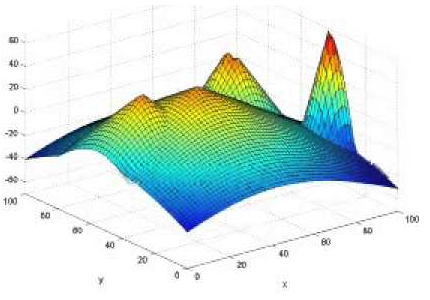
\includegraphics[scale=0.5]{images/moving_peak.png}
	\label{fig:moving_peaks}{\\Fonte: \citeonline{moving_peak_1999}.}
\end{figure}

\subsection{Ocillating Peaks}

O \textit{benchmark} de oscilação de picos (\textit{ocillating peaks}) é baseado no de movimentação de picos, porem foi desenvolvido para algoritmos evolutivos com utilização de memória.

É uma combinação linear entre duas funções, em que o peso delas altera ao longo do tempo, portanto, a função $G$, começa em $g_1$, passa para $g_2$, depois volta para $g_1$ e assim sucessivamente. Em outras palavras o máximo absoluto de $G$ oscila entre dois pontos $g_1$ e $g_2$. Basicamente essa função se relaciona com o problema da mochila oscilatória que tem visto tantos exemplos bem sucedidos de abordagens evolutivas baseados em memória.

As funções que representam as alteração da função $G$ estão representadas na Equação \ref{eq:ocillating_peak_alterations}, em que, $\lambda (t)$ representa a oscilação da função, $n$ é a soma das picos das duas funções que compõem a combinação linear e $m$ é o número de dimensões.

\begin{equation}
\label{eq:ocillating_peak_alterations}
\begin{split}
& \delta \in N(0,1) \\
& \lambda (t) = \frac{\cos{\frac{2\pi t}{100\delta}} +1}{2} \\
& g_1(\vec{x}) = \sum_{i=1}^{n/_2} \frac{H_i}{1+W_i \sum_{j=1}^{m} (x_j - X_j(t))^2} \\
& g_2(\vec{x}) = \sum_{i=n/_2+1}^{n} \frac{H_i}{1+W_i \sum_{j=1)}^{m} (x_j - X_j(t))^2} \\
& G(t,\vec{x}) = \lambda (t) g_1(\vec{x}) + (1-\lambda (t))g_2(\vec{x})
\end{split}
\end{equation}

